\section{Minimalizacja wskaźnika jakości regulacji}
W celu doboru parametrów modelu wykorzystano optymalizacjeę poprzez funkcję $fmincon$ programu MATLAB, 
jako parametr optymalizacji wybrano wskaźnika jakości regulacji $E$.

\begin{figure}[H]
    \centering
    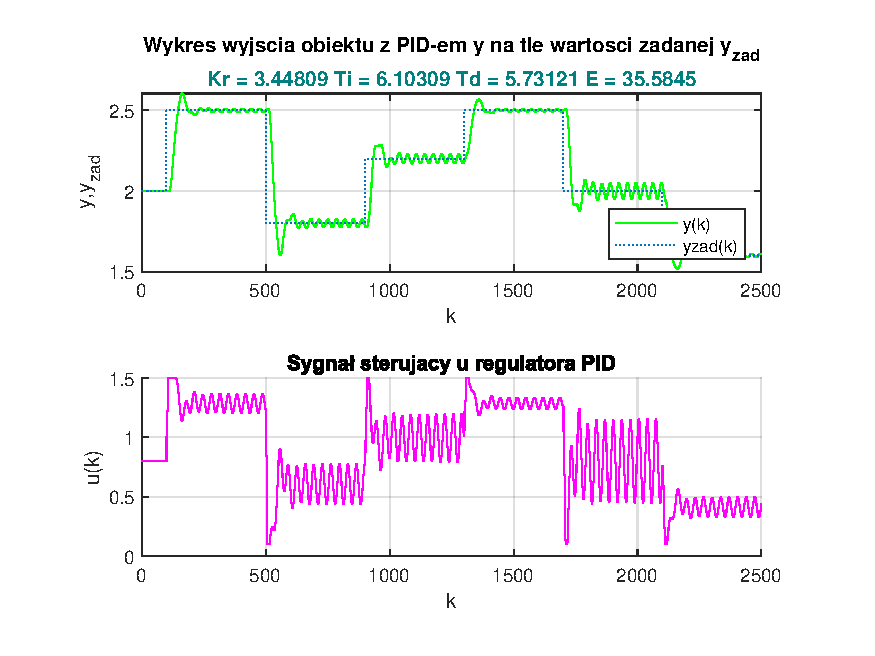
\includegraphics[scale=0.90]{../projekt/zad6/PID_opt_pdf/PID_opt.pdf}
    \caption{Regulator PID z optymalizacji}
\end{figure}

\begin{figure}[H]
    \centering
    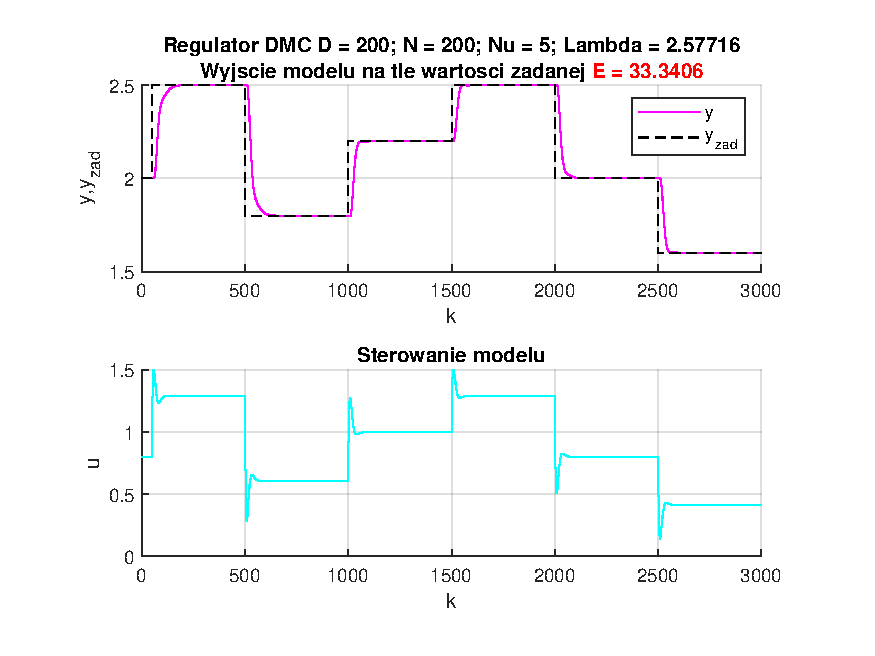
\includegraphics[scale=0.90]{../projekt/zad6/DMC_opt_pdf/DMC_opt.pdf}
    \caption{Regulator DMC z optymalizacji}
\end{figure}
